\documentclass{beamer}
\usepackage{graphicx}
\usepackage{amsmath,amssymb,amsfonts}
\usepackage[utf8]{inputenc}

\hypersetup{
    colorlinks=true, % Activate colors for links
    linkcolor=blue,  % Internal links color
    urlcolor=blue,   % External links color
    citecolor=blue   % Citation links color
}

\title{Credit Card Fraud Detection}
\subtitle{Project for Fraud Detection Course}
\author{Ricardo Araújo Amorim \\ up202107843}
\institute{}
\date{December 12, 2024}

% Custom footer with title and group ID
\setbeamertemplate{footline}{%
  \leavevmode%
  \hbox{%
  \begin{beamercolorbox}[wd=1\paperwidth,ht=2.25ex,dp=1ex,leftskip=1em,rightskip=1em]{author in head/foot}%
    \usebeamerfont{author in head/foot}\insertshorttitle\hfill\insertpagenumber
  \end{beamercolorbox}}%
}

% Remove navigation symbols
\setbeamertemplate{navigation symbols}{}

\begin{document}
\small

% Title Slide
\begin{frame}
    \titlepage
\end{frame}

% Slide 1: Project Overview
\begin{frame}{Project Overview}
    \begin{itemize}
        \item \textbf{Objective:} Detect fraudulent credit card transactions using machine learning.
        \item \textbf{Steps in the Process:}
        \begin{itemize}
            \item Data Understanding.
            \item Data Preparation.
            \item Clustering.
            \item Modeling.
            \item Evaluation and Results.
        \end{itemize}
        \item \textbf{Challenges:}
        \begin{itemize}
            \item Highly imbalanced dataset (fraud cases = 1.9\%).
            \item Complex interactions between features.
        \end{itemize}
    \end{itemize}
\end{frame}

% Slide 2: Data Understanding
\begin{frame}{Data Understanding: Overview}
    \begin{columns} % Create two columns
        \begin{column}{0.6\textwidth}
        \begin{itemize}
            \item Some attributes were converted to the \texttt{object} type for better handling during data preparation and modeling.
            \item \textbf{Changed Attributes:}
            \begin{itemize}
                \item \texttt{index}: Changed to \texttt{object}.
                \item \texttt{cc\_num}: Changed to \texttt{object}.
                \item \texttt{is\_fraud}: Changed to \texttt{object}.
                \item \texttt{zip}: Changed to \texttt{object}.
                \item \texttt{merchant\_id}: Changed to \texttt{object}.
            \end{itemize}
        \end{itemize}
        \end{column}

      \begin{column}{0.4\textwidth}
        \begin{figure}
            \centering
            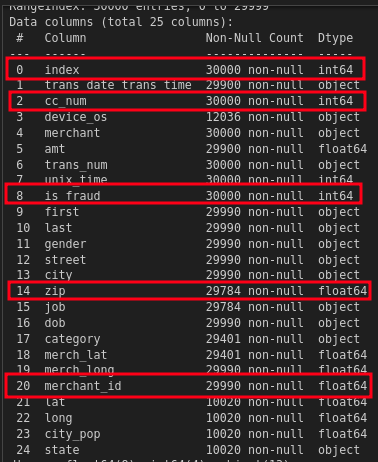
\includegraphics[width=1\textwidth]{images/dataset.png} % Replace with your image file
            \caption{Original Dataset}
        \end{figure}
        \end{column}
    \end{columns}
\end{frame}

% Slide 3: Correlation Matrix
\begin{frame}{Correlation Matrix}
    \begin{columns} % Create two columns
        % First column: Text
        \begin{column}{0.5\textwidth}
            \textbf{Key Insights:}
            \begin{itemize}
                \item Analyzed numerical features for linear relationships.
                \item Most features show weak or no correlation.
                \item Significant correlations observed:
                \begin{itemize}
                    \item \texttt{unix\_time} and \texttt{index}.
                    \item \texttt{city\_pop} with \texttt{lat} and \texttt{long}.
                \end{itemize}
            \end{itemize}
        \end{column}
        
        % Second column: Image
        \begin{column}{0.5\textwidth}
            \begin{figure}
                \centering
                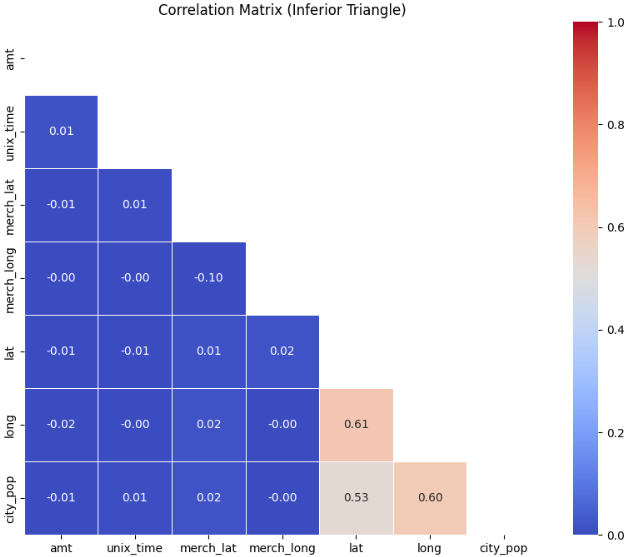
\includegraphics[width=1\textwidth]{images/corr.png} % Replace with your correlation matrix image file
                \caption{Correlation Matrix}
            \end{figure}
        \end{column}
    \end{columns}
\end{frame}

% Slide 4: Chi-Square Test Results
\begin{frame}{Chi-Square Test Results}
    \begin{columns} % Create two columns
        % First column: Text
        \begin{column}{0.5\textwidth}
            \textbf{Key Insights:}
            \begin{itemize}
                \item Tested independence among categorical variables.
                \item Significant dependencies found:
                \begin{itemize}
                    \item \texttt{gender} and \texttt{dob}.
                    \item \texttt{job} and \texttt{merchant}.
                \end{itemize}
                \item Highlighted relationships guided feature engineering.
                \item Created new interaction variables (e.g., \texttt{job\_age\_group}).
            \end{itemize}
        \end{column}
        
        % Second column: Image
        \begin{column}{0.5\textwidth}
            \begin{figure}
                \centering
                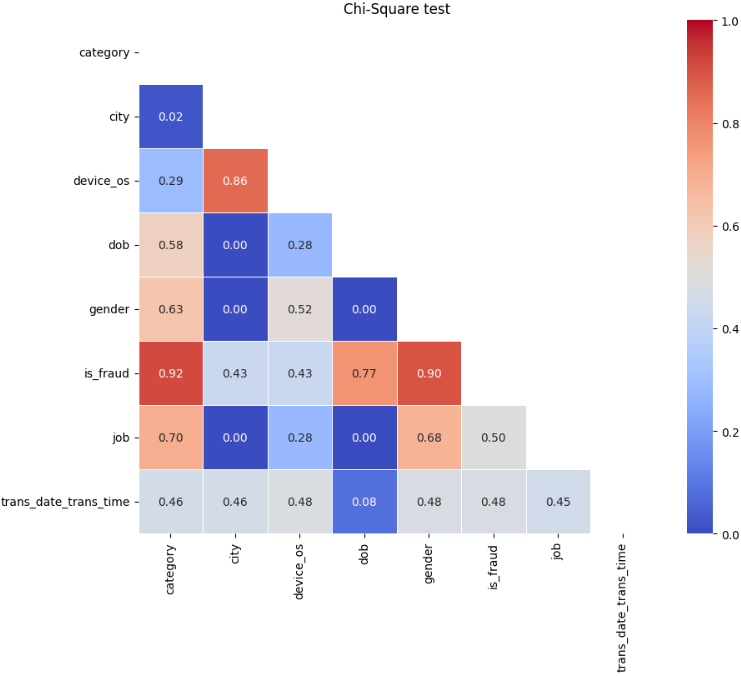
\includegraphics[width=1\textwidth]{images/chi.png} % Replace with your Chi-Square matrix image file
                \caption{Chi-Square Test Results}
            \end{figure}
        \end{column}
    \end{columns}
\end{frame}

% Slide 5: Transaction Amount Distribution
\begin{frame}{Data Visualization}
    \begin{columns} % Create two columns
        % First column: Text
        \begin{column}{0.5\textwidth}
            \begin{figure}
                \centering
                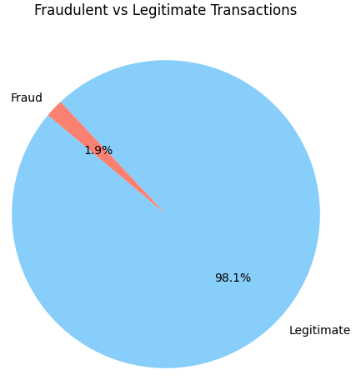
\includegraphics[width=0.7\textwidth]{images/fraudvsleg.png} % Replace with your transaction amount distribution image file
                \caption{Fraudulent vs Legitimate Transactions}
            \end{figure}
        \end{column}
        
        % Second column: Image
        \begin{column}{0.5\textwidth}
            \begin{figure}
                \centering
                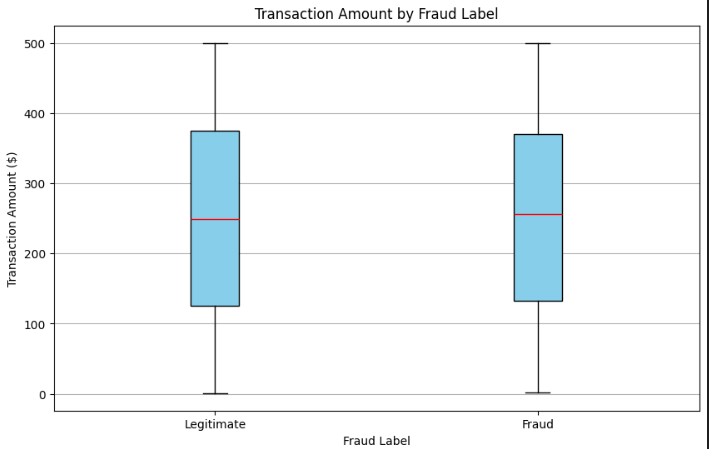
\includegraphics[width=1\textwidth]{images/amt.png} % Replace with your transaction amount distribution image file
                \caption{Transaction Amount Distribution}
            \end{figure}
        \end{column}
    \end{columns}
\end{frame}

\begin{frame}{Data Visualization}
    \begin{columns} % Create two columns
        % First column: Text
        \begin{column}{0.5\textwidth}
            \begin{figure}
                \centering
                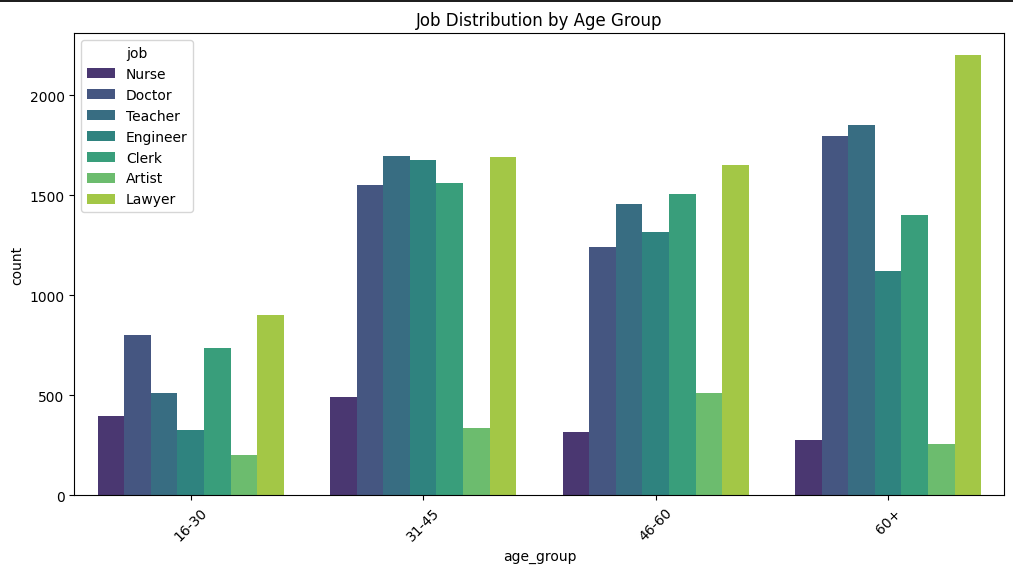
\includegraphics[width=1\textwidth]{images/jog_age.png} % Replace with your transaction amount distribution image file
                \caption{Job Distribution by Age Group}
            \end{figure}
        \end{column}
        
        % Second column: Image
        \begin{column}{0.5\textwidth}
            \begin{figure}
                \centering
                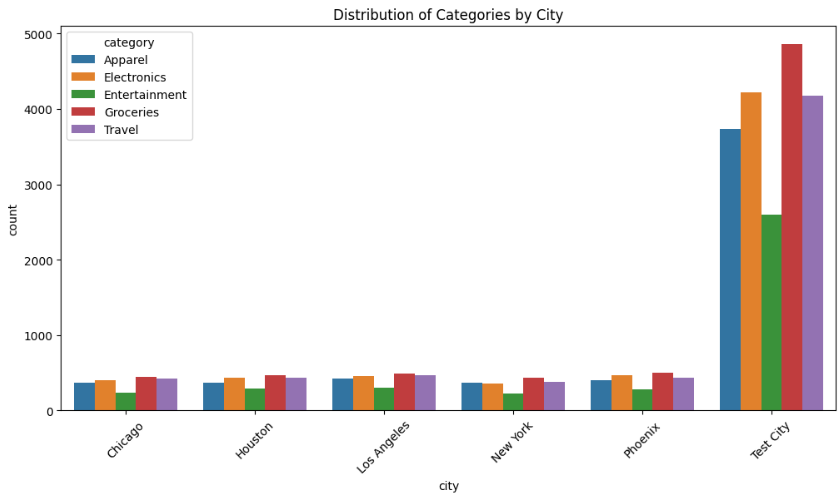
\includegraphics[width=1\textwidth]{images/city.png} % Replace with your transaction amount distribution image file
                \caption{Distribution of Categories by City}
            \end{figure}
        \end{column}
    \end{columns}
\end{frame}

\begin{frame}{Data Visualization}
    \begin{columns} % Create two columns
        % First column: Text
        \begin{column}{0.5\textwidth}
            \begin{figure}
                \centering
                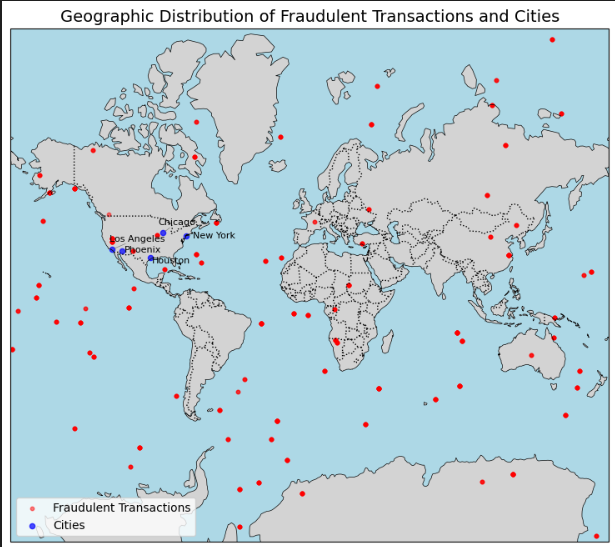
\includegraphics[width=1\textwidth]{images/mapa.png} % Replace with your transaction amount distribution image file
                \caption{Geographic Distribution of Fraudulent Transactions}
            \end{figure}
        \end{column}
        
        % Second column: Image
        \begin{column}{0.5\textwidth}
            \begin{figure}
                \centering
                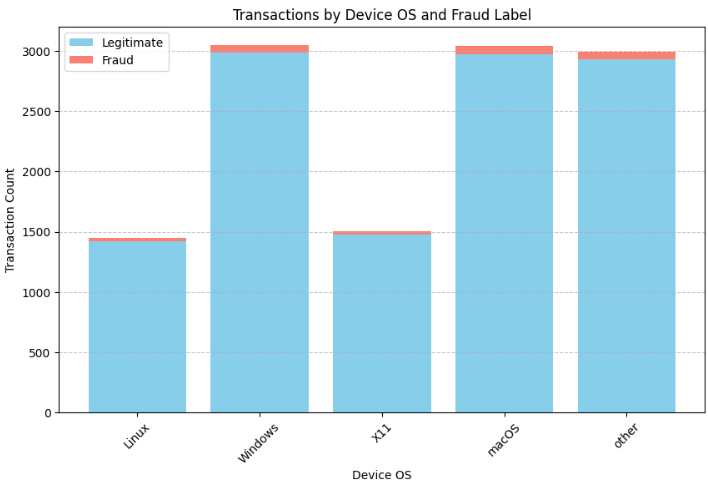
\includegraphics[width=1\textwidth]{images/device.png} % Replace with your transaction amount distribution image file
                \caption{Transactions by Device OS and Fraud Label }
            \end{figure}
        \end{column}
    \end{columns}
\end{frame}

% Slide 3: Data Preparation
\begin{frame}{Data Preparation}
    \begin{itemize}
        \item \textbf{Dataset Split:}
        \begin{itemize}
            \item Divided into 80\% training and 20\% testing datasets.
            \item Used \textbf{stratification} to ensure the same proportion of fraud and non-fraud transactions in both sets.
            \item Maintains the balance of the target variable (\texttt{is\_fraud}) for better model performance and evaluation.
        \end{itemize}
        \item \textbf{Handling Duplicates:}
        \begin{itemize}
            \item Transaction number (\texttt{trans\_num}) must be unique to maintain data integrity.
            \item Identified duplicate transaction numbers and retained only the record with fewer missing values (NAs).
        \end{itemize}
    \end{itemize}
\end{frame}


% Slide 4: Feature Engineering
\begin{frame}{Feature Engineering}
    \begin{itemize}
        \item \textbf{Age and Age Group Creation:}
        \begin{itemize}
            \item Calculated \texttt{age} by subtracting the date of birth (\texttt{dob}) from the transaction date (\texttt{unix\_time}).
            \item Grouped \texttt{age} into categorical \texttt{age\_group}:
            \begin{itemize}
                \item Bins: \textit{16–30}, \textit{31–45}, \textit{46–60}, \textit{60+}.
            \end{itemize}
        \end{itemize}
        \item \textbf{Interaction Features:}
        \begin{itemize}
            \item Combined \texttt{age\_group} with \texttt{job} to create interaction variables (\texttt{job\_age\_group}).
        \end{itemize}
        \item \textbf{Cyclical Temporal Features:}
        \begin{itemize}
            \item Derived \texttt{hour\_sin}, \texttt{hour\_cos} for the hour of the day.
            \textbf{Benefits:}
            \begin{itemize}
                \item Encodes the proximity of hours (e.g., 23:00 and 00:00 are close).
                \item Improves model performance by providing meaningful temporal patterns.
            \end{itemize}
        \end{itemize}
    \end{itemize}
\end{frame}

% Slide: Dropped Attributes
\begin{frame}{Dropped Attributes}
    \begin{itemize}
        \item During data preparation, several attributes were removed to improve model efficiency and focus on relevant features.
        \item \textbf{Reasons for Removal:}
        \begin{itemize}
            \item \textbf{Redundancy:}
            \begin{itemize}
                \item \texttt{index}, \texttt{trans\_num}: Added no predictive value, purely identifiers.
                \item \texttt{trans\_date\_trans\_time}, \texttt{transaction\_date}: Replaced by derived features like \texttt{hour\_sin}, \texttt{hour\_cos}
            \end{itemize}
            \item \textbf{Privacy Concerns:}
            \begin{itemize}
                \item \texttt{first}, \texttt{last}, \texttt{street}, \texttt{state}, \texttt{dob}, \texttt{cc\_num}: Contained personal or sensitive information.
            \end{itemize}
        \end{itemize}
    \end{itemize}
\end{frame}

% Slide 3: Data Preparation
\begin{frame}{Dropped Attributes}
    \begin{itemize}
        \item \textbf{Low Predictive Value:}
        \begin{itemize}
            \item \texttt{lat}, \texttt{long}, \texttt{merch\_lat}, \texttt{merch\_long}: Geographic data did not significantly correlate with fraud.
            \item \texttt{zip}, \texttt{merchant}, \texttt{merchant\_id}: Low variance or redundancy with other features.
        \end{itemize}
        \item \textbf{Replaced by Derived Features:}
        \begin{itemize}
            \item \texttt{age}: Replaced by \texttt{age\_group}.
    \end{itemize}
    \end{itemize}
\end{frame}

\begin{frame}{Handling Missing Values}
    \begin{itemize}
        \item \textbf{Training Data:}
        \begin{itemize}
            \item \textbf{Numeric Variables:}
            \begin{itemize}
                \item Missing values imputed using the \textbf{k-Nearest Neighbors (kNN)} algorithm:
                \begin{itemize}
                    \item Numeric columns standardized before applying \texttt{kNN}.
                    \item Post-imputation, values re-scaled to their original distributions using stored \texttt{mean} and \texttt{standard deviation}.
                \end{itemize}
            \end{itemize}
    \item \textbf{Categorical Variables:}
            \begin{itemize}
                \item Handled automatically by \texttt{kNN}, using the \textbf{mode of the nearest neighbors}.
            \end{itemize}
            \item Final dataset saved as \texttt{X\_train\_without\_missing\_values.csv}.
        \end{itemize}

    \end{itemize}
\end{frame}

\begin{frame}{Handling Missing Values}
    \begin{itemize}
        \item \textbf{Testing Data:}
        \begin{itemize}
            \item \textbf{Numeric Variables:}
            \begin{itemize}
                \item Imputed using the \textbf{mean values} computed from the training dataset.
            \end{itemize}
        \item \textbf{Categorical Variables:}
            \begin{itemize}
                \item Imputed using the \textbf{mode values} from the training dataset.
            \end{itemize}
        \end{itemize}
        Ensured consistency by aligning imputed values with the training dataset.
\end{itemize}
\end{frame}

% Slide: One-Hot Encoding
\begin{frame}{One-Hot Encoding}
    \begin{itemize}
        \item \textbf{Purpose:}
        \begin{itemize}
            \item Convert categorical variables into a numerical format suitable for machine learning models.
        \end{itemize}
        \item \textbf{Process:}
        \begin{itemize}
            \item Identified categorical columns using \texttt{select\_dtypes}.
            \item Applied \textbf{one-hot encoding} to transform these columns:
            \begin{itemize}
                \item Used \texttt{drop\_first} for binary categories to avoid multicollinearity.
                \item Retained all categories for non-binary columns.
            \end{itemize}
            \item Ensured the same encoding scheme was applied to both training and testing datasets.
        \end{itemize}
        \item \textbf{Output:}
        \begin{itemize}
            \item Each categorical column was replaced with multiple binary columns representing the categories.
        \end{itemize}
    \end{itemize}
\end{frame}



% Slide: Normalization and Scaling
\begin{frame}{Normalization and Scaling}
    \begin{columns} % Create two columns
        % First column: Text
    \begin{column}{0.6\textwidth}
    \begin{itemize}
        \item \textbf{Purpose:}
        \begin{itemize}
            \item Normalize numerical variables to ensure all features have comparable scales.
            \item Prevent variables with larger ranges from dominating the model.
        \end{itemize}
        \item \textbf{Why MinMaxScaler?}
        \begin{itemize}
            \item Chosen because the distribution of numerical variables is not uniform.
            \item Scales values to a specified range, typically \([0, 1]\), preserving the original shape of the data distribution.
        \end{itemize}
    \end{itemize}
    \end{column}

    \begin{column}{0.4\textwidth}
    \begin{figure}
        \centering
        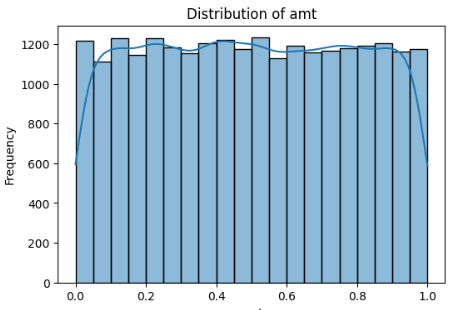
\includegraphics[width=1\textwidth]{images/norm.png} % Replace with an appropriate image
        \caption{Distribution of \texttt{amt} attribute}
    \end{figure}
\end{column}
\end{columns}
\end{frame}


% Slide 5: Modeling Approach
\begin{frame}{Normalization and Scaling}
    \begin{itemize}
        \item \textbf{Benefits of Scaling:}
        \begin{itemize}
            \item Improves the performance of distance-based algorithms (e.g., k-Nearest Neighbors, clustering).
            \item Ensures gradient-based optimization algorithms converge faster and more reliably.
            \item Helps prevent bias in models sensitive to variable magnitude.
        \end{itemize}
    \end{itemize}
\end{frame}

% Slide: Clustering Overview
\begin{frame}{Clustering Overview}
    \begin{itemize}
        \item \textbf{Objective:}
        \begin{itemize}
            \item Group transactions based on their similarity using unsupervised learning.
        \end{itemize}
        \item \textbf{Features Used for Clustering:}
        \begin{itemize}
            \item \texttt{amt}: Transaction amount.
            \item \texttt{hour\_sin}, \texttt{hour\_cos}: Temporal features representing the hour of the transaction.
            \item \texttt{city\_pop}: Population size of the city where the transaction occurred.
        \end{itemize}
        \item \textbf{Clustering Techniques Explored:}
        \begin{itemize}
            \item \textbf{DBSCAN (Density-Based Spatial Clustering of Applications with Noise)}.
            \item \textbf{K-Means Clustering}.
        \end{itemize}
    \end{itemize}
\end{frame}

% Slide: DBSCAN Clustering
\begin{frame}{DBSCAN Clustering}
    \begin{columns} % Create two columns
        % First column: Text
    \begin{column}{0.6\textwidth}
    \begin{itemize}
        \item \textbf{Approach:}
        \begin{itemize}
            \item Identifies clusters based on density of points.
            \item Parameters used:
            \begin{itemize}
                \item \texttt{eps}: 0.5 (maximum distance between points in a cluster).
                \item \texttt{min\_samples}: 2 (minimum points to form a dense region).
            \end{itemize}
        \end{itemize}
    \end{itemize}
    \end{column}

    \begin{column}{0.4\textwidth}
    \begin{figure}
        \centering
        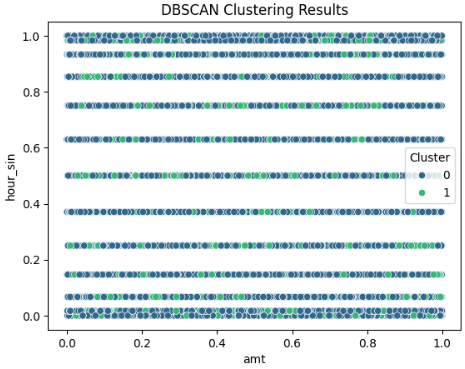
\includegraphics[width=1\textwidth]{images/dbscan.png} % Replace with the DBSCAN scatterplot
        \caption{DBSCAN Clustering Results}
    \end{figure}
\end{column}
\end{columns}
\end{frame}


% Slide: K-Means Clustering
\begin{frame}{K-Means Clustering}
        \begin{columns} % Create two columns
        % First column: Text
    \begin{column}{0.6\textwidth}
    \begin{itemize}
        \item \textbf{Approach:}
        \begin{itemize}
            \item Groups data into \texttt{k} clusters by minimizing the within-cluster variance.
            \item Tested different values of \texttt{k} (2 to 10) to find the best clustering structure.
        \end{itemize}
    \end{itemize}
    \end{column}

    \begin{column}{0.4\textwidth}
    \begin{figure}
        \centering
        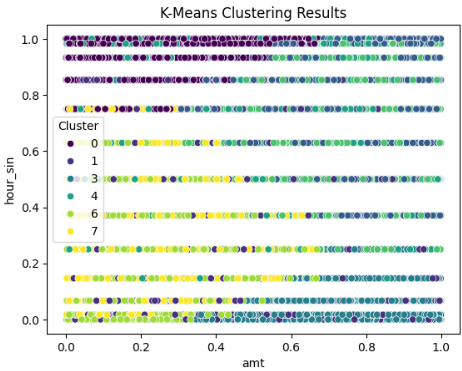
\includegraphics[width=1\textwidth]{images/kmeans.png} % Replace with the K-Means scatterplot
        \caption{K-Means Clustering Results (Best \texttt{k})}
    \end{figure}
\end{column}
\end{columns}
\end{frame}


% Slide: Handling Class Imbalance
\begin{frame}{Handling Class Imbalance}
    \begin{itemize}
        \item \textbf{Class Imbalance:}
        \begin{itemize}
            \item The dataset exhibits significant class imbalance:
            \begin{itemize}
                \item Majority class: \texttt{is\_fraud = 0}.
                \item Minority class: \texttt{is\_fraud = 1}.
            \end{itemize}
            \item Imbalance can lead to biased models with poor recall for fraud detection.
        \end{itemize}
        \item \textbf{Solution:} 
        \begin{itemize}
            \item Combined \textbf{SMOTE (Synthetic Minority Oversampling)} and \textbf{RandomUnderSampling}.
            \item SMOTE increases minority class representation by generating synthetic samples.
            \item RandomUnderSampling reduces majority class size, balancing the dataset and preventing computational overhead.
        \end{itemize}
    \end{itemize}
\end{frame}

% Slide: Why SMOTE + RandomUnderSampling?
\begin{frame}{Why SMOTE + RandomUnderSampling?}
    \begin{itemize}
        \item \textbf{Comparison with SMOTE-Tomek:}
        \begin{itemize}
            \item SMOTE-Tomek removes Tomek links (overlapping samples between classes).
            \item Analysis showed no significant class overlap, making SMOTE-Tomek less relevant.
        \end{itemize}
        \item \textbf{Advantages of SMOTE + RandomUnderSampling:}
        \begin{itemize}
            \item Simpler and faster than SMOTE-Tomek.
            \item Balances the dataset without unnecessary removal of data points.
        \end{itemize}
        \item \textbf{Oversampling and Undersampling Rates:}
        \begin{itemize}
            \item Oversampling rates tested: \texttt{0.5, 0.7} (fractions of the majority class).
            \item Undersampling rates tested: \texttt{0.8, 0.9} (fractions of the total dataset for the majority class).
        \end{itemize}
    \end{itemize}
\end{frame}

% Slide: Model Pipeline
\begin{frame}{Model Pipeline}
    \begin{itemize}
        \item \textbf{Pipeline Steps:}
        \begin{enumerate}
            \item Apply \textbf{SMOTE} for oversampling the minority class.
            \item Apply \textbf{RandomUnderSampling} to balance the dataset.
            \item Train the model on the balanced dataset.
        \end{enumerate}
        \item \textbf{Evaluation Metrics:}
        \begin{itemize}
            \item \textbf{Precision:} Accuracy of fraud predictions.
            \item \textbf{Recall:} Ability to detect fraudulent transactions.
            \item \textbf{F1-Score:} Balance between precision and recall.
            \item \textbf{AUC-ROC:} Overall performance across classification thresholds.
        \end{itemize}
    \end{itemize}
\end{frame}

% Slide: Hyperparameter Tuning with Random Search
\begin{frame}{Hyperparameter Tuning: Random Search}
    \begin{itemize}
        \item \textbf{Objective:} Improve model performance by finding the best combination of hyperparameters.
        \item \textbf{Why Random Search?}
        \begin{itemize}
            \item More efficient than Grid Search for large hyperparameter spaces.
            \item Allows exploring a wide range of combinations with fewer iterations.
        \end{itemize}
        \item \textbf{Implementation:}
        \begin{itemize}
            \item Used \texttt{RandomizedSearchCV} with 5-fold cross-validation.
            \item \textbf{What is 5-fold cross-validation?} A technique to evaluate model performance by splitting the data into 5 equally sized subsets, or "folds."
            \item Evaluated models based on the \textbf{AUC-ROC} score to handle class imbalance effectively.
        \end{itemize}
    \end{itemize}
\end{frame}

% Slide: Models Overview (Part 1)
\begin{frame}{Models Overview}
    \begin{itemize}
        \item \textbf{Random Forest:}
        \begin{itemize}
            \item Ensemble-based model combining multiple decision trees.
            \item Effective for imbalanced datasets and interpretable results.
        \end{itemize}
    \begin{figure}
        \centering
        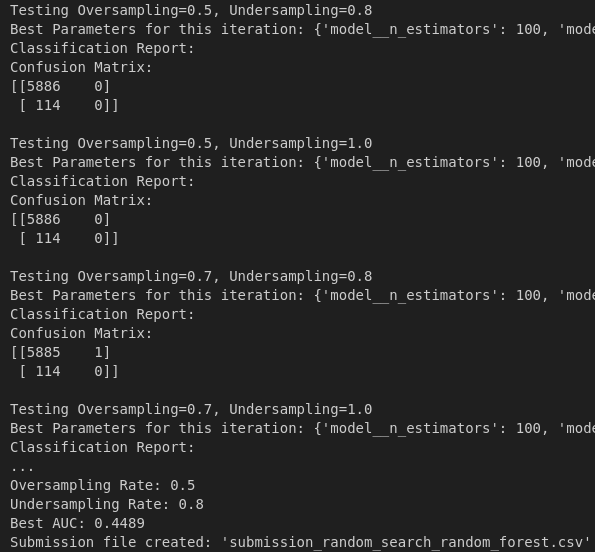
\includegraphics[width=0.4\textwidth]{images/rf.png} % Replace with an image showing MLP and SVM visuals
        \caption{Random Forest Results Overview}
    \end{figure}

    \end{itemize}
\end{frame}

\begin{frame}{Models Overview}
        \item \textbf{XGBoost:}
        \begin{itemize}
            \item Gradient boosting framework optimized for speed and performance.
            \item Excellent at capturing complex, non-linear patterns in data.
        \end{itemize}
    \begin{figure}
        \centering
        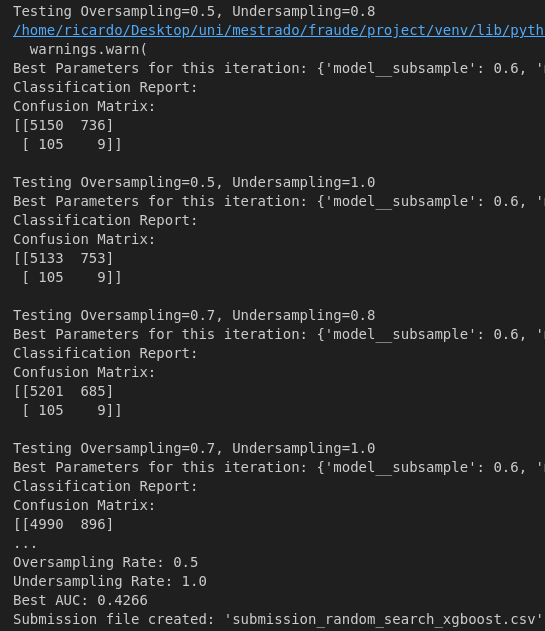
\includegraphics[width=0.4\textwidth]{images/xgb.png} % Replace with an image showing MLP and SVM visuals
        \caption{XGBoost Results Overview}
    \end{figure}
\end{frame}

\begin{frame}{Models Overview}
        \item \textbf{Decision Tree (Best AUC-ROC Score):}
        \begin{itemize}
            \item Simple and interpretable tree-based model.
            \item Tends to overfit but works well with proper pruning and parameter tuning.
        \end{itemize}
    \begin{figure}
        \centering
        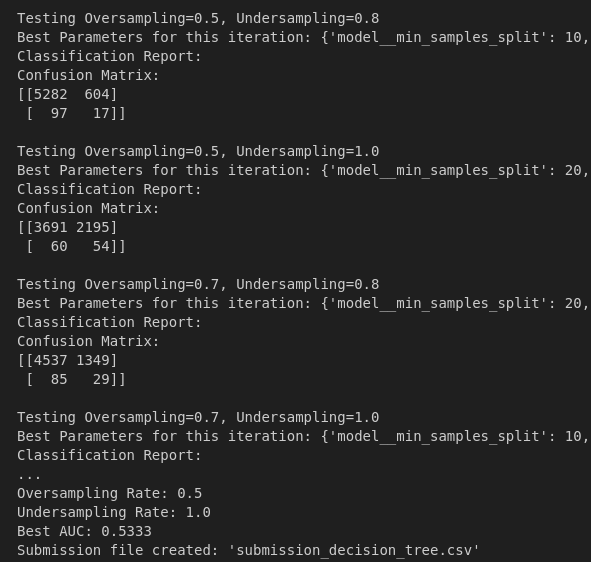
\includegraphics[width=0.5\textwidth]{images/dt.png} % Replace with an image showing MLP and SVM visuals
        \caption{Decision Tree Results Overview}
    \end{figure}
\end{frame}

% Slide: Models Overview (Part 2)
\begin{frame}{Models Overview}
    \begin{itemize}
        \item \textbf{Multi-Layer Perceptron (MLP):}
        \begin{itemize}
            \item Neural network model with hidden layers.
            \item Effective for capturing non-linear relationships in data.
        \end{itemize}
    \begin{figure}
        \centering
        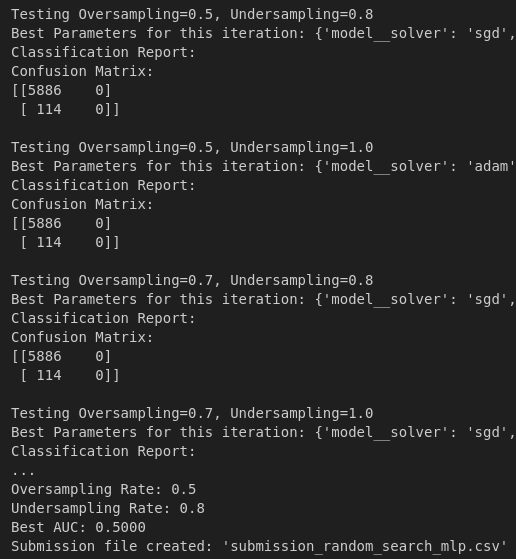
\includegraphics[width=0.45\textwidth]{images/mlp.png} % Replace with an image showing MLP and SVM visuals
        \caption{MLP Results Overview}
    \end{figure}
    \end{itemize}
\end{frame}

\begin{frame}{Models Overview}
        \item \textbf{Support Vector Machine (SVM):}
        \begin{itemize}
            \item Separates data using hyperplanes in high-dimensional space.
            \item Effective for smaller datasets and well-separated classes.
        \end{itemize}
    \begin{figure}
        \centering
        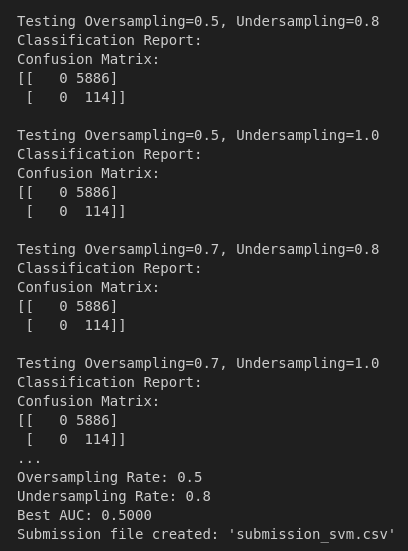
\includegraphics[width=0.4\textwidth]{images/svm.png} % Replace with an image showing MLP and SVM visuals
        \caption{SVM Results Overview}
    \end{figure}
\end{frame}

% Slide 7: Conclusion
\begin{frame}{Conclusion}
    \begin{itemize}
        \item The \textbf{Decision Tree} performed the best, but with modest results.
        \item Valuable insights were gained by following systematic steps.
        \item The approach shows potential for better outcomes with real-world data.
    \end{itemize}
\end{frame}


% Slide 8: Questions
\begin{frame}{}
    \centering
    Thank you for your attention! \\
\end{frame}

\end{document}

